\subsection{Analysis of Interviews}

The answers given during the three group interviews has been summarized and clustered into three areas, see figure \ref{fig:overview}. Further, the answers within interaction design has been clustered into its four main principles, see figure \ref{fig:interactiondesign}. The questions regarding learning has tried to answer why a coach is correct or incorrect on a given question, see figure \ref{fig:learning}. Service design has been clustered into the two questions "When do you want to use the app?" and "When are you not able to use the app?", see figure \ref{fig:servicedesign}. Zoomed-in versions of all of the areas are presented after the overviews, where the analysis of the quotes can be seen in its fullest. The quotes from these mind-maps are individual, which means that if another coach has had a similar thought, their quote is branched next to the following quote.

\begin{figure}[h]
    \centering
    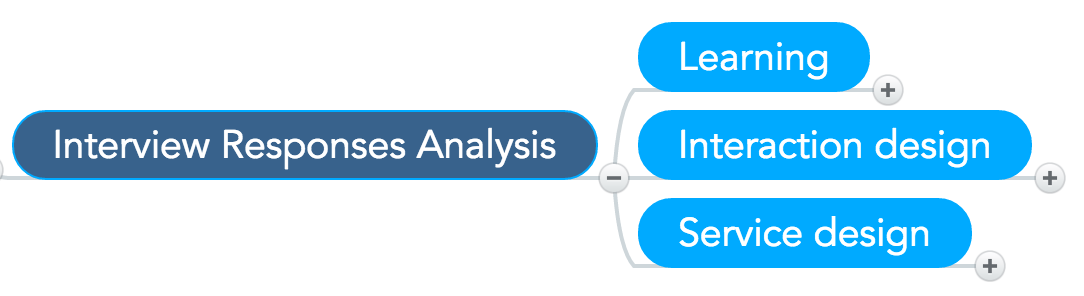
\includegraphics[width=0.3\textwidth]{analysis/interviews/overview_notexpanded.png}
    \caption{The interview answers has been clustered into three areas: learning, interaction design and service design.}
    \label{fig:overview}
\end{figure}

\begin{figure}[h]
    \centering
    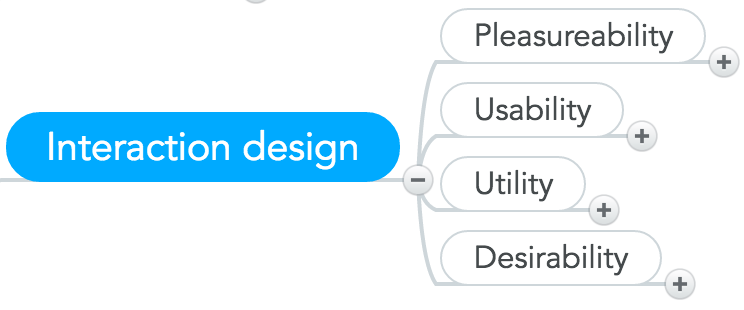
\includegraphics[width=0.3\textwidth]{analysis/interviews/interactiondesign_notexpanded.png}
    \caption{The coach quotes regarding interaction design have been divided by four criteria: pleasurability, usability, utility and desirability.}
    \label{fig:interactiondesign}
\end{figure}

%For learning and service design, the analysis of the interview quotes can bee seen in its fullest in figure \ref{fig:learning} and figure \ref{fig:servicedesign} respectively. Zoomed-in versions of all of the areas are presented after the overviews, where the analysis of the quotes can be seen in its fullest.

\begin{figure}[h]
    \centering
    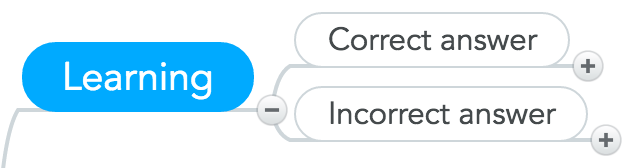
\includegraphics[width=0.3\textwidth]{analysis/interviews/learning_notexpanded.png}
    \caption{The coach quotes regarding learning have been divided by if they give insight to why a coach has been correct or incorrect on a given question.}
    \label{fig:learning}
\end{figure}

\begin{figure}[h]
    \centering
    
\includegraphics[width=0.3\textwidth]{analysis/interviews/servicedesign_notexpanded.png}
    \caption{The coach quotes regarding service design have been divided into \textit{when} you want to use the YoungDrive app, and when you are hindered from doing so.}
    \label{fig:servicedesign}
\end{figure}

\clearpage

\subsubsection{Learning}\label{sec:interview-learning}

By reading the quotes from the coaches carefully, it can be understood why answers can appear correct by the coaches (see figure \ref{fig:learning1}), even if this would not be the case (see figure \ref{fig:learning2}.

\begin{figure}[h]
    \centering
    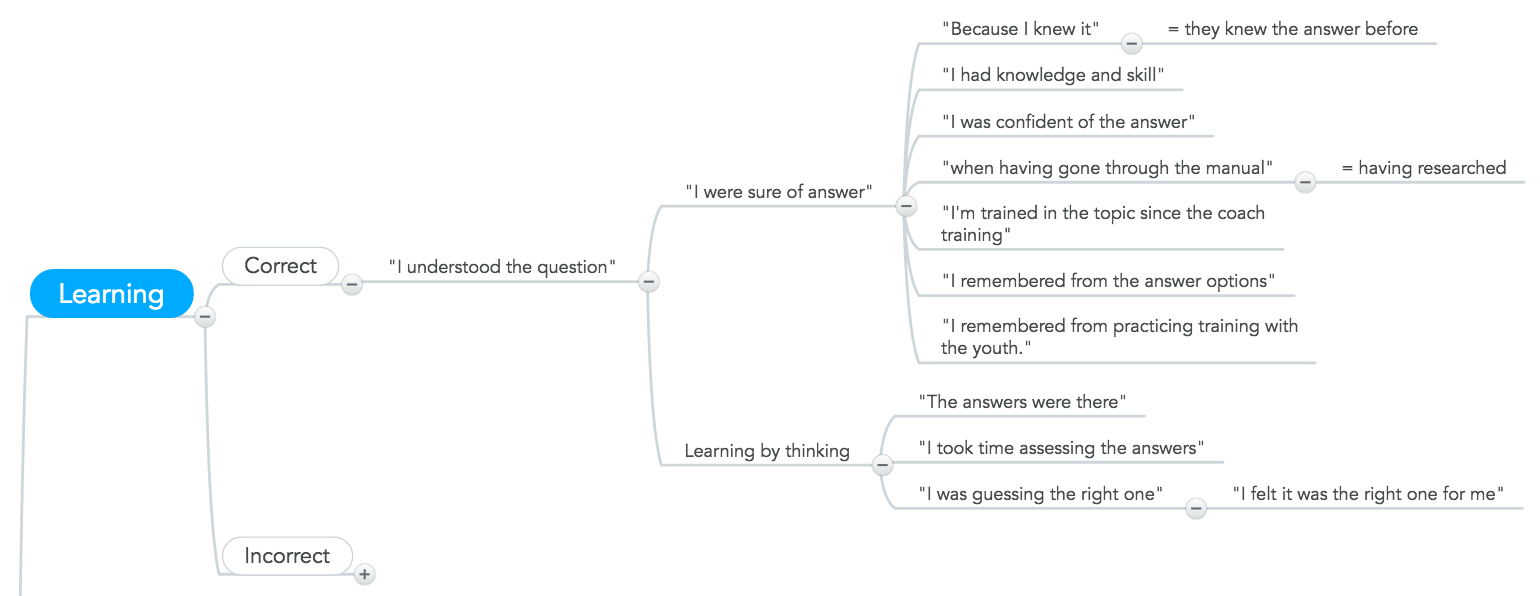
\includegraphics[width=1.0\textwidth]{analysis/interviews/learning_correct.png}
    \caption{Quotes explaining why a coach could give a correct answer to a given question. Either you were sure of the answers, or you made a qualified guess. A prerequisite for answering the question correctly is that you understood the question's meaning.}
    \label{fig:learning1}
\end{figure}

\begin{figure}[h]
    \centering
    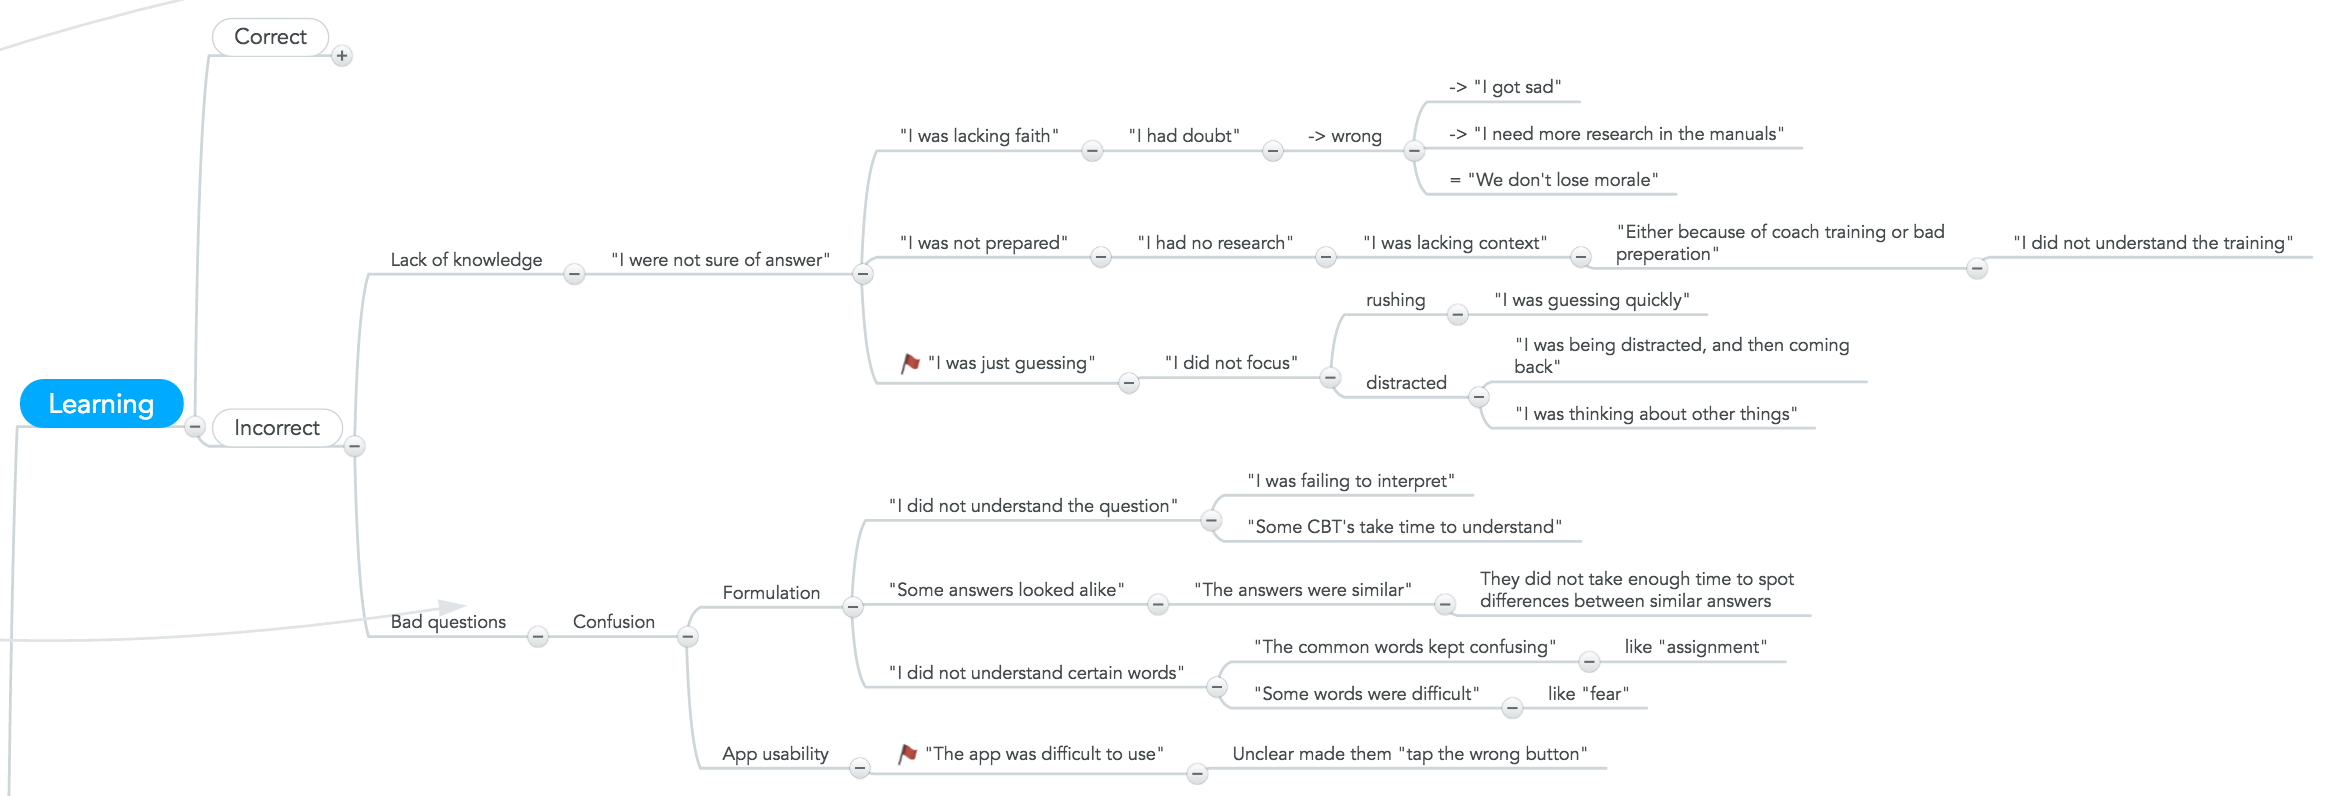
\includegraphics[width=1.0\textwidth]{analysis/interviews/learning_incorrect.png}
    \caption{Quotes explaining why a coach could give an incorrect answer on a given question. Either, the coach did not have sufficient knowledge to answer the question confidently (for a number of reasons, given in the figure), or the question was not understood correctly, or the app usability was a hindrance.}
    \label{fig:learning2}
\end{figure}

\clearpage

\subsubsection{Interaction Design}

Most importantly, in the final app test, everyone thought the app was good and easy to use (n = 26). This is important, as this had not been the case in iteration 3. Regarding the four different areas of interaction design, positive remarks on utility are especially beneficial for learning. However, pleasurability, usability and desirability is a prerequisite for the app to be used by the coaches. For desirability, if the coaches are stimulated by using the app, two reviews were: "It felt good using the app" and "It motivated learning". The other three interaction principles (pleasurability, usability and utility) have been given their own mind-map below, see figure \ref{fig:interaction1}, figure \ref{fig:interaction2} and \ref{fig:interaction3}.

\begin{figure}[h]
    \centering
    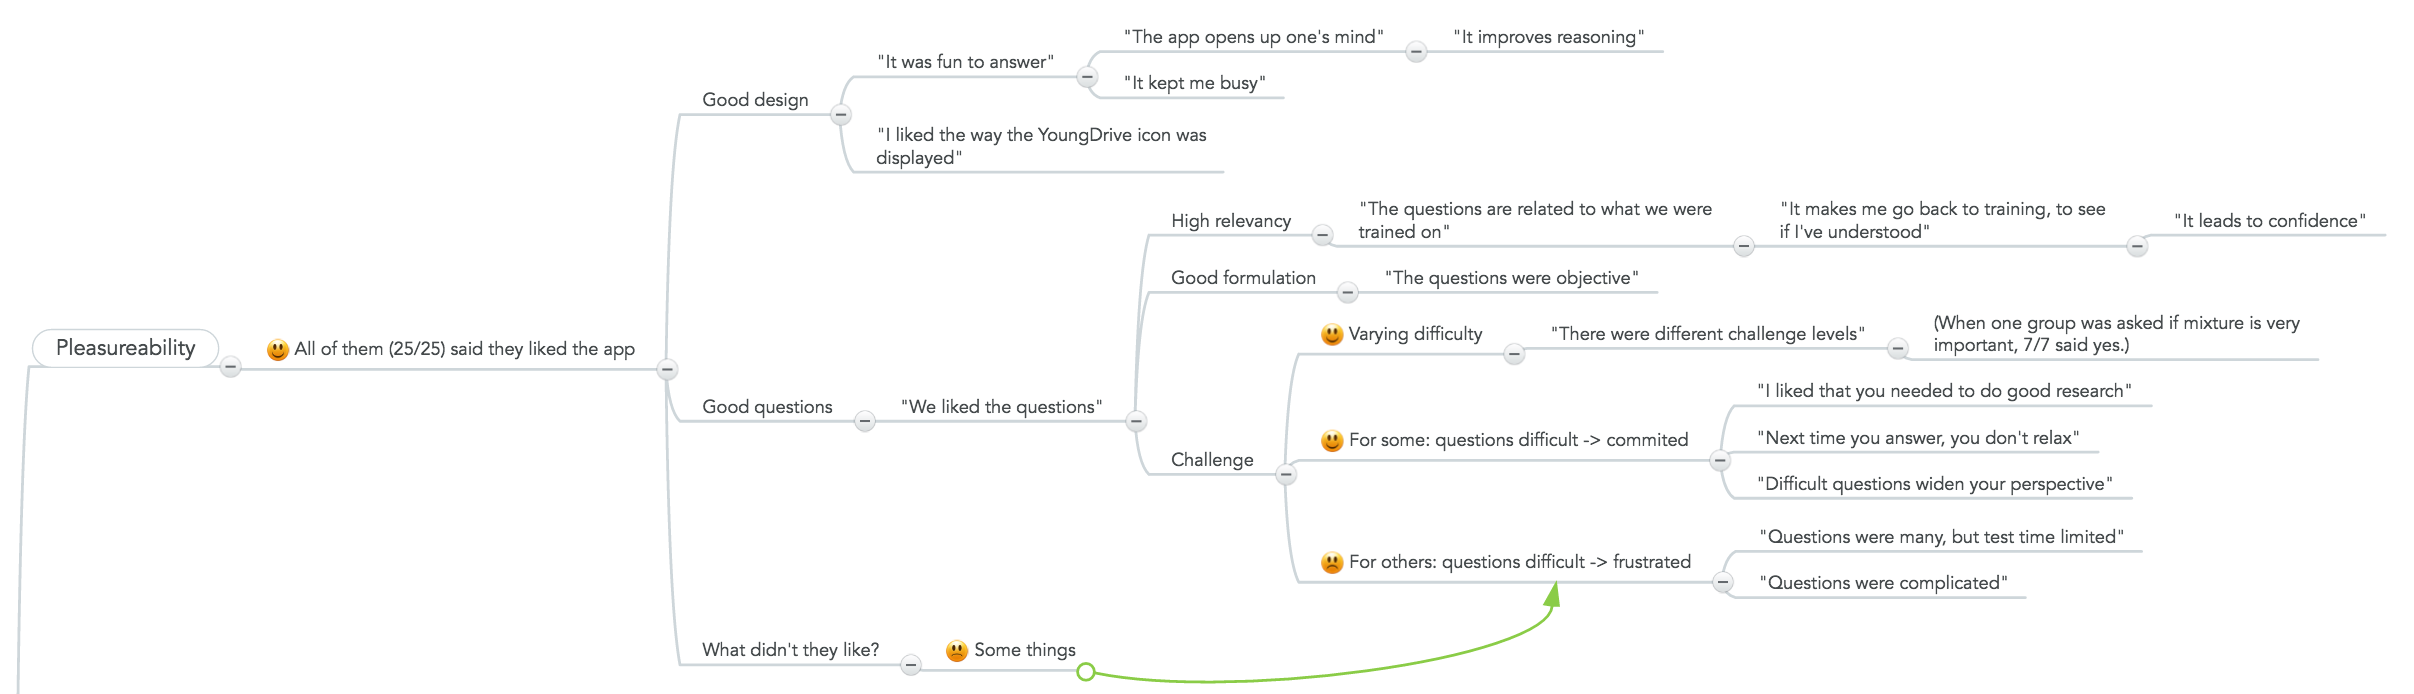
\includegraphics[width=1.0\textwidth]{analysis/interviews/interactiondesign_pleasurability.png}
    \caption{Pleasurability was 100\%, as the app had a good design and well-motivated questions, however some coaches were frustrated by difficult questions in the app, or the time needed to complete a quiz during the workshop.}
    %From the interviews, it is visible that the coaches feel the quizzes has been a fair way to measure their knowledge in the topic. The answer "It leads to confidence" could show that when a coach has done a quiz reaching certification, they do feel more confident about teaching the topic.
    %Positively, assessment of "Am I ready?" can happen already before the youth session, in the app.}
    \label{fig:interaction1}
\end{figure}

\begin{figure}[h]
    \centering
    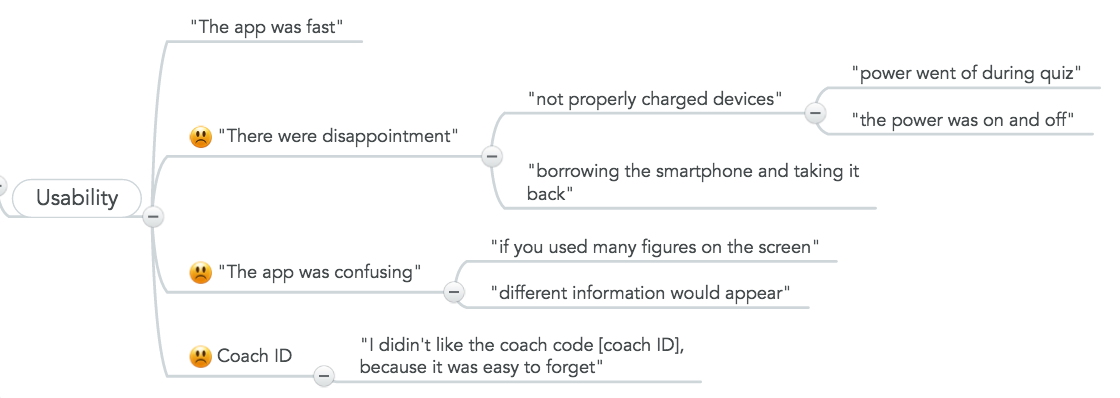
\includegraphics[width=1.0\textwidth]{analysis/interviews/interactiondesign_usability.png}
    \caption{Usability. As previosuly stated, all of the coaches (25/25) thought the app was easy to use when asked by raise of hands. However, in the interviews, some detailed comments regarding usability appeared. Regarding workshop issues, some of the devices' battery died during the workshop, or needed to be replaced. Regarding the app, some still mention too much information to appear at once, or that information are shown that the coach does not expect. Only one coach mentioned thinking that thee login was not user friendly, since the Coach ID was easy to forget. The Coach ID has since been documented by the local project leaders, so they can be contacted in such situations.}
    \label{fig:interaction2}
\end{figure}

\begin{figure}[h]
    \centering
    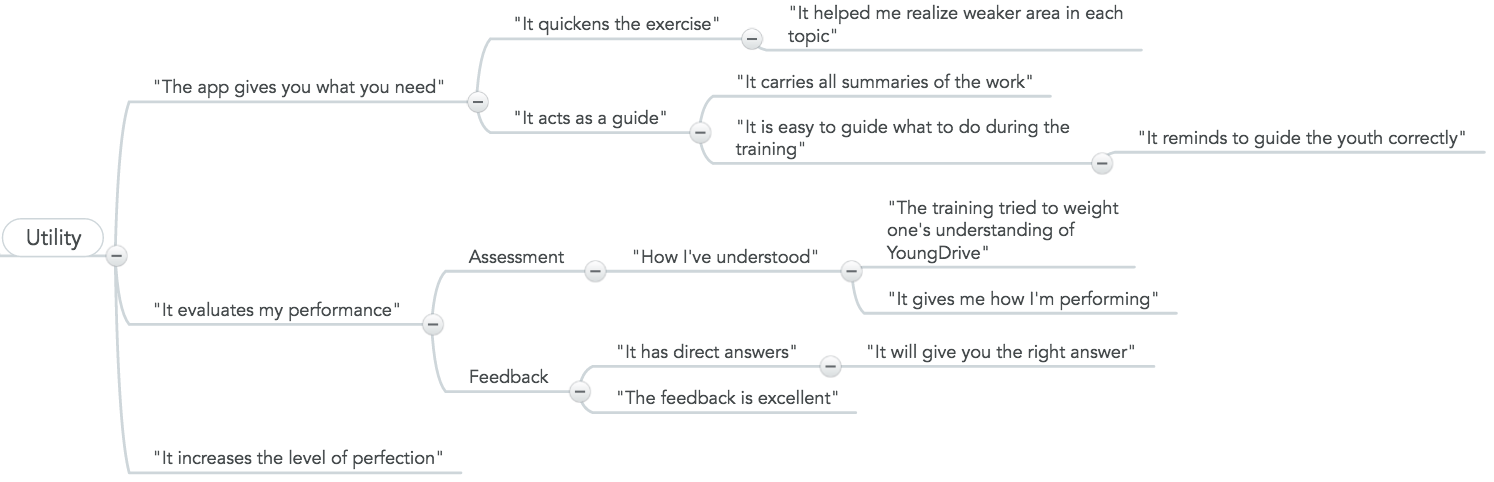
\includegraphics[width=1.0\textwidth]{analysis/interviews/interactiondesign_utility.png}
    \caption{Utility gives a valuable measure of what benefits the coach finds with using the app. Quotes regarding usefulness are: "It quickens the exercise", "It carries all summaries of the work", "It reminds to guide the youth correctly". For training, coaches conclude that "It evaluates my performance" and that "The feedback is excellent". One coach summarizes with "It increases the level of perfection".}
    \label{fig:interaction3}
\end{figure}

\clearpage

\subsubsection{Service Design}

It is important to understand if and when the app will be used by the coach, and if the environment of the coach in any way can hinder use of the app. For understanding the coach situation to these two criteria, see figure \ref{fig:servicedesign1} and \ref{fig:servicedesign1}.

\begin{figure}[h]
    \centering
    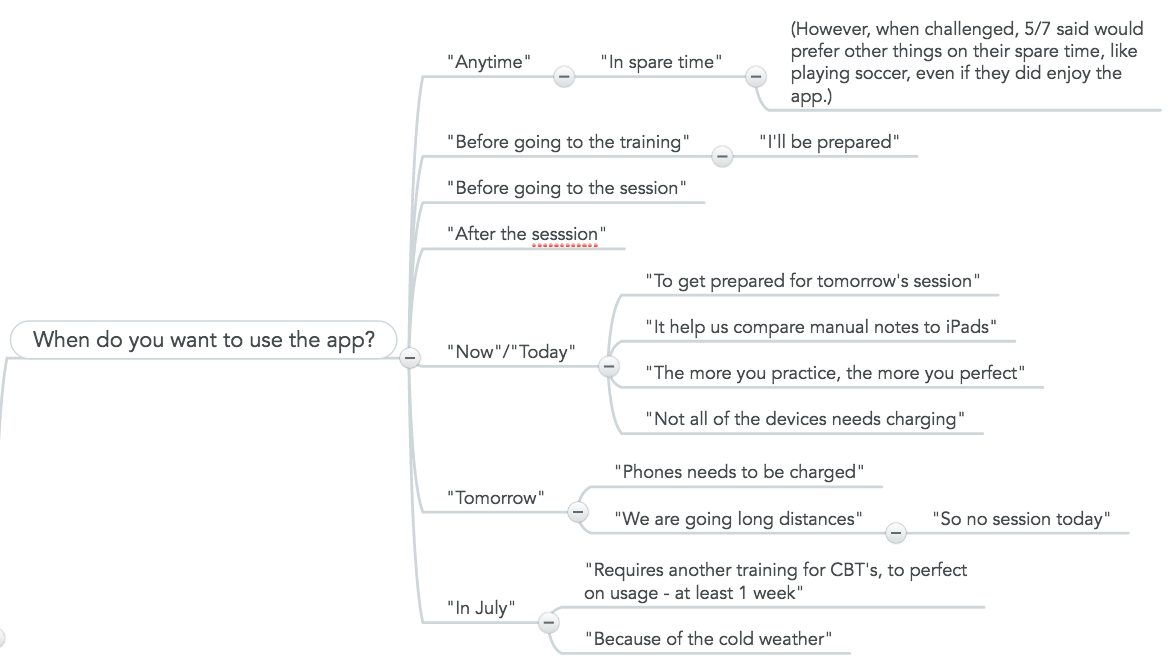
\includegraphics[width=1.0\textwidth]{analysis/interviews/servicedesign_when.png}
    \caption{There are very varying answers to the question "When do you want to use the app?". Most coaches would have liked to use the app immediately. Some of the coaches identified the need for devices, more training, or charging of devices in being able to do so.}
    \label{fig:servicedesign1}
\end{figure}

\begin{figure}[h]
    \centering
    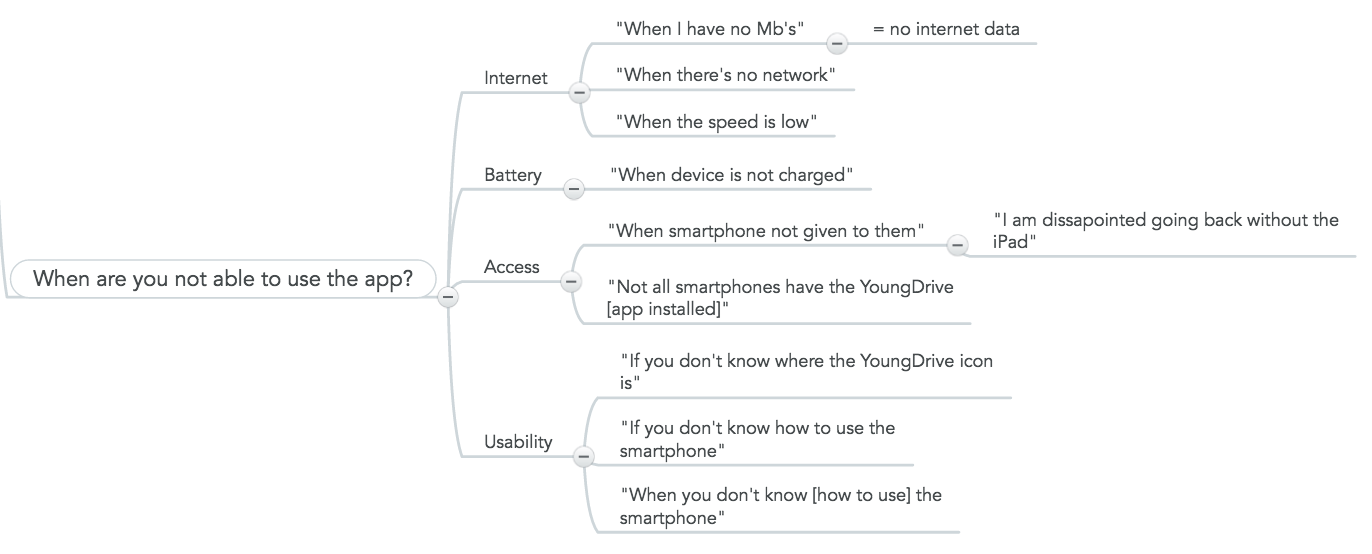
\includegraphics[width=1.0\textwidth]{analysis/interviews/servicedesign_cant.png}
    \caption{Answers for the question "When are you not able to use the app?" are grouped into four segments: internet issues, battery issues, low or no access to smartphones, or if the app is not usable because it is not available on the smartphone, or the coach does not know how to use a smartphone.}
    \label{fig:servicedesign2}
\end{figure}

\clearpage
